\documentclass[12pt,a4paper]{report}

\usepackage[francais]{babel}
\usepackage[utf8]{inputenc}
\usepackage{epigraph}
\usepackage[T1]{fontenc}
\usepackage{listings}
\usepackage{graphicx}
\usepackage{parskip}
\usepackage{xcolor}


%% config
\definecolor{deepblue}{rgb}{0,0,0.5}

\graphicspath{{images/}}
\lstset{
	literate={à}{{\`a}}1,
    language={Python},
    basicstyle=\ttfamily\small, 
    tabsize=4,
    keywordstyle=\bold,
    commentstyle=\color{gray},
    backgroundcolor=\color{lightgray},
    otherkeywords={self},
	keywordstyle=\ttfamily\small\color{deepblue},
    frame=single
    showtabs=false,
    showspaces=false,
    showstringspaces=false
}

\renewcommand{\labelitemi}{∙}
%%macro

\newcommand{\path}[1]{\texttt{#1}}

\newcommand{\codeintext}[1]{\texttt{#1}}

\begin{document}


\title{{\huge Inititation à la programmation}}
\author{Bastien Gorissen \& Thomas Stassin}
\date{Année 2016}

\maketitle
%% \tableofcontents

\chapter{Level 1}
\begin{figure}[ht]
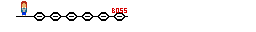
\includegraphics[scale=1]{stage_0.png} 
\end{figure}

\section{Qu’est-ce qu’un langage de programmation?}

\epigraph{Un langage de programmation est une convention pour donner des ordres à un ordinateur. Ce n’est pas censé être obscur, bizarre et plein de pièges subtils.
Ca, ce sont les caractéristiques de la magie.}{\textit{Dave Small}}

Un langage de programmation est un moyen d’intéragir avec l’ordinateur afin de lui donner des instructions, le langage qui est \emph{intelligible}, 
sera \emph{interprété} afin d’être compris par la machine.

\begin{figure}[ht]
\centering
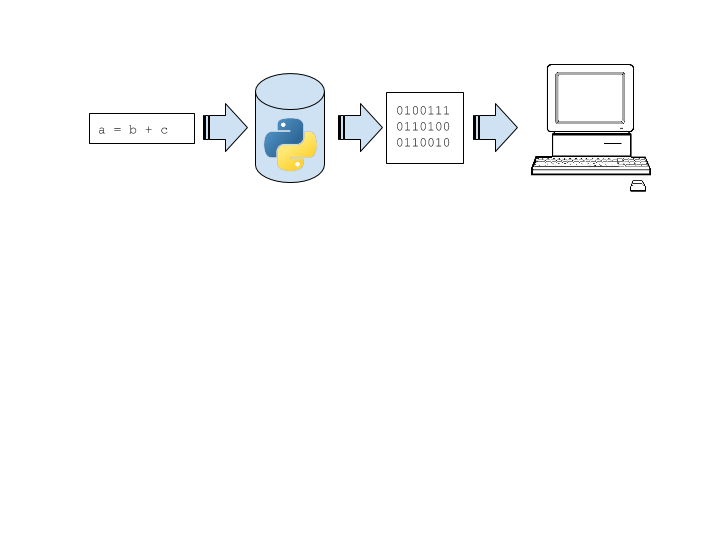
\includegraphics[scale=0.5]{translate_code.png} 
\end{figure}

\subsection{Commentaires}

Si vous ouvrez le script \path{run\_game.py}, vous pourrez voir que certaines lignes commencent par \codeintext{\#}. Celles-ci seront ignorées par l'ordinateur. Ce sont des \emph{commentaires} destinés à clarifier le code.

\subsection{Stage 1-1}
\begin{figure}[ht]
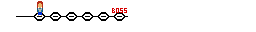
\includegraphics[scale=1]{stage_1.png} 
\end{figure}

Exécuter le script se trouvant dans le dossier \path{lv1/run\_game.py}

\section{Commander à l'ordinateur}

Pour ``commander'' l’ordinateur, on lui donne des \emph{instructions}, le plus souvent, ces instructions seront regroupées dans un \emph{script}.

\subsection{Stage 1-2}
\begin{figure}[ht]
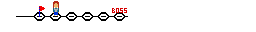
\includegraphics[scale=1]{stage_2.png} 
\end{figure}

Dans l’exercice précédent, nous avons exécuté le script \path{run\_game.py}, ce script est rempli d’instructions, dont celles-ci:

\begin{lstlisting}
    dungeon_size = (5, 5)
    game = world.Game(dungeon_size)
    game.run()
\end{lstlisting}

Que ce passerait-il si on modifiait l’instruction qui définit la grandeur du donjon dans le script ?
Changez les données de dimension du donjon dans le script et observez ce qu'il se passe lors de l'exécution du script.

\subsection{\`{A} retenir}

Python est un \emph{langage sensible à la casse}\footnote{\textit{Case sensitive} en anglais.}, ce qui veut dire qu'il fait la différence entre les majuscules et les minuscules. Autrement dit \codeintext{A} sera différent de \codeintext{a} et \codeintext{world} différent de \codeintext{World}.

Donc si je remplace \codeintext{world} par \codeintext{World} dans le script précédent, il générera une erreur.

\begin{lstlisting}
    dungeon_size = (5, 5)
    game = World.Game(dungeon_size)
    game.run()
\end{lstlisting}

Vous devriez obtenir un message ressemblant à ``\codeintext{NameError: name 'World' is not defined}''

\section{Les instructions de sortie}

Il existe plusieurs sortes d’instructions, l’une d’elles sont les instructions de sortie.
Une instruction de sortie envoie vers une “sortie” ce qu’on lui donne.
Une des sorties les plus couramment utilisée est la console et avec Python, l’instruction de sortie vers la console est \codeintext{print}.

Et donc voici le classique, mais indémodable “Hello World” en Python :

\begin{lstlisting}
    print("Hello World!")
\end{lstlisting}


\subsection{Stage 1-3}
\begin{figure}[ht]
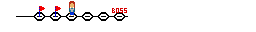
\includegraphics[scale=1]{stage_3.png} 
\end{figure}

Lorsque le donjon est créé, signalez-le par un message dans la \emph{console}.

\section{Les variables}

Souvent, il sera utile de stocker certaines valeurs tout au long de l’exécution de votre code.
Par exemple pour stocker la valeur d’un calcul, ou même afin de réutiliser ses valeurs plusieurs fois. Pour stocker des valeurs, on utilise des \emph{variables}.

La \emph{variable} est un moyen de stocker une valeur quelconque (un nombre, du texte, voire même des \emph{objets} plus complexes) dans la mémoire du programme.

Dans le cas de notre jeu, le donjon, ainsi que le héro sont contenus chacun dans une \emph{variable}.

\begin{lstlisting}
dungeon_size = (5, 5)
game = world.Game(dungeon_size)
hero = Game.hero
\end{lstlisting}

En Python, l’\emph{affectation} d’une valeur se fait avec l’opérateur \emph{=}.

Dans \codeintext{a=3}, on affecte \codeintext{3} à la variable \codeintext{a}\footnote{ En Python il suffit d’affecter une valeur à une variable pour qu’elle commence à exister, ce n’est pas vrai pour la plupart des langages (comme le C\# par exemple).}

\subsection{Stage 1-4}
\begin{figure}[ht]
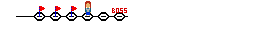
\includegraphics[scale=1]{stage_4.png} 
\end{figure}

Faites en sorte de stocker les dimensions du donjon dans des variables (par exemple \codeintext{length} et \codeintext{width}\footnote{Il est courant d'utiliser des noms de variables en anglais. La programmation est un monde très anglophone.}).

\section{Opérations sur une chaîne de caractères}

Il vous sera parfois utile de savoir manipuler des chaînes de caractères, l'exemple classique est dans une ligne de dialogue, où l'on voudrait dire au héros le nombre d'ennemis qu'il lui reste à tuer avant de finir la quête. Or, lorsque que vous codez, vous ne connaissez pas le nombre d'ennemis. Vous avez sûrement stocké cette information dans une variable et donc vous allez devoir intégrer cette variable à votre ligne de dialogue.

\subsection{Conversion}
Il y un moyen facile de convertir une variable en chaine de caractères\footnote{En Python les chaines de caractères ont le \emph{type} \codeintext{str} pour le mot anglais \textit{string}, qui veut dire chaîne}, il suffit d'utiliser la fonction \codeintext{str}.

Si je voulais convertir la variable \codeintext{nbr\_enemies} qui contient le chiffre \codeintext{3} je procéderais comme suit:

\begin{lstlisting}
	nbr_enemies = 3
	nbr_enemies = str(nbr_enemies)
\end{lstlisting}

A la fin de l'exécution de ce petit script, \codeintext{nbr\_enemies} ne vaut plus \codeintext{3} mais \codeintext{"3"}.

\subsection{Concaténation}
Le fait de coller deux chaînes de caractères l'une derrière l'autre porte un nom: \emph{la concaténation}.
En Python, l'opérateur pour \emph{concaténer} deux variables ensemble est l'opérateur \codeintext{+}.

Par exemple, si je voulais concaténer la variable contenant le nom du héro avec un message cela donnerait :
 
\begin{lstlisting}
	message = ", il te reste des ennemis à tuer."
	message = hero_name + message
\end{lstlisting}

Donc si le héro se nomme Brutor, la chaîne de caractères en fin de script sera égale à \codeintext{"Brutor, il te reste des ennemis à tuer."}

On peut même aller plus loin en mêlant la \emph{conversion} et la \emph{concaténation} en indiquant aussi dans le message le nombre d'ennemis qu'il reste.

\begin{lstlisting}
	message = ", il te reste " + str(nbr_enemies)"
	message = message + " ennemis à tuer."
	message = hero_name + message
\end{lstlisting}

\subsection{Stage 1-5}
\begin{figure}[ht]
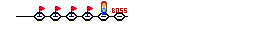
\includegraphics[scale=1]{stage_5.png} 
\end{figure}

Lorsque le donjon est créé, indiquer dans un message à la console la longueur et la largeur de celui-ci.

\section{Les fonctions et les méthodes, première approche}

Pour terminer ce premier level, on va mettre des mots sur deux choses que l'on a vues précédemment. Les \emph{fonctions globales} et les \emph{méthodes}.
Nous avons déjà vu plusieurs fonctions dans les parties précédentes:
\begin{itemize}
	\item[$\bullet$] \codeintext{print}
	\item[$\bullet$] \codeintext{str}
\end{itemize}

Ces fonctions sont dîtes "globales". Ce type de fonctions n'est pas lié à un type d'\emph{objet}.

Il existe aussi une série de fonctions liées à des \emph{objets}, par exemple la fonction \emph{run} de la variable \emph{game}.
On appelle ces fonctions des \emph{méthodes} et elles sont liées à un type d'objets en particulier.

\subsection{Stage 1-6}
\begin{figure}[ht]
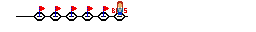
\includegraphics[scale=1]{stage_6.png} 
\end{figure}

La variable du héros, sobrement appelée \codeintext{hero} est du type \codeintext{Hero}, c'est un type de variable que nous avons construit pour le jeu\footnote{Nous verrons plus tard qu'il est possible de définir ses propres types et de leur donner les caractéristiques que l'on désire.}. Nous avons donné trois \emph{méthodes} à cette variable:

\begin{description}
	\item[\codeintext{turn\_left}:] ce qui fait tourner le héros à gauche.
	\item[\codeintext{turn\_right}:] ce qui fait tourner le héros à droite.
	\item[\codeintext{move}:] ce qui fait avancer le héros d'une "case".
\end{description}

Essayez de faire bouger le héros grâce à ces trois méthodes.

\section{Bonus Stage}
\begin{figure}[ht]
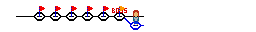
\includegraphics[scale=1]{stage_bonus.png} 
\end{figure}

Pour compléter le stage bonus il faut que vous arriviez à amener le héros sur la sortie du donjon. La sortie est représentée par la case bleue en haut à gauche de la pièce.
Le donjon doit au moins avoir une longueur et une largeur de 7.

\end{document}